\documentclass[jou,12pt,a4paper]{apa6}

%%%%%%%%%%%%%%%%%%%% Loading packages %%%%%%%%%%%%%%%%%%%% 
\usepackage{csquotes}
\usepackage[american]{babel}
\usepackage{amsmath, amssymb, graphicx,gensymb}
\usepackage{fixltx2e} % Misc Latex fixes
\usepackage{url}
\usepackage{threeparttable}
\usepackage{anyfontsize}
\usepackage{adjustbox}
\usepackage{subfigure}
\usepackage{threeparttable}
\usepackage{tabularx}
\usepackage[capposition=top]{floatrow}
\usepackage[colorlinks=true,citecolor=blue,urlcolor=red,draft]{hyperref}
\usepackage{apacite}
\usepackage{courier}

%%%%%%%%%%%%%%%%%%%% Set some paramters %%%%%%%%%%%%%%%%%%
\setlength{\parindent}{10mm}
\setlength{\parskip}{0mm}
\graphicspath{ {Figures/} } % path to images

%%%%%%%%%%%%%%%%%%%% Title and such %%%%%%%%%%%%%%%%%%%%%%
\title{\LARGE On the dimensionality of neural representations}
\shorttitle{Dimensionality of neural representations}

\author{Lukas Snoek}
\affiliation{University of Amsterdam}
\authornote{Lukas Snoek, student nr. 10126228, University of Amsterdam, Email: lukassnoek@gmail.nl.}

%%%%%%%%%%%%%%%%%%%%%%%%%%%%%%%%%%%%%%%%%%%%%%%%%%%%%%%%%
%  OPTIONAL STUFF  									
%	\leftheader{Snoek}		ONLY IN [jou] MODE			
%	\journal{Journal of Awesomeness}					
%	\volume{2(3)}										
%	\note{version 1}									
%%%%%%%%%%%%%%%%%%%%%%%%%%%%%%%%%%%%%%%%%%%%%%%%%%%%%%%%%

\abstract{The brain is organized anatomically and functionally at different scales, from ensembles of neurons within cortical columns to interacting regions in networks spanning the entire brain. Multivariate pattern analysis (MVPA) is an increasingly popular method to investigate how information is represented neurally, but little is known how information is represented at these different levels of organization in the brain. Often, MVPA studies restrict their analyses to local patterns of voxels, thus assuming a localized, voxel-level representation of information. While this local organization is neurobiologically plausible for representations of low-level psychological concepts such as visual stimulus-features, studies on high-level psychological concepts such as emotion, motivation, and decision-making suggest that these are encoded at a larger spatial scale within globally distributed functional networks. The current study aims at investigating the spatial scale and dimensionality of high-level representations, using existing data from a study investigating the representation of self-focused emotion experience. We hypothesized that we could accurately model these high-level neural representations as a multivariate set of clusters, instead of local voxel patterns, using a linear classifier. Results demonstrated that high-level representations could indeed be accurately modeled at cluster-level. However, additional exploratory analyses showed that, in addition to cluster-level networks, the investigated high-level representations were also encoded locally as voxel-level patterns in multiple spatially-contiguous regions in the brain, suggesting a multiscale organization of information. We believe that our study shows that high-level representations should be analyzed at different spatial scales in the brain, as it may give insight into different sources of information.}

%%%%%%%%%%%%%%%%%%%% Begin doc! %%%%%%%%%%%%%%%%%%%%
\begin{document}

%%%%%%%%%%%%%%%%%%%% Titlepage! %%%%%%%%%%%%%%%%%%%%
% Original template from:  http://www.latextemplates.com/template/university-assignment-title-page
% which is drawn from https://en.wikibooks.org/wiki/LaTeX/Title_Creation.

\begin{titlepage}

\newcommand{\HRule}{\rule{\linewidth}{0.5mm}} 
\center 

% Headings
\textsc{\LARGE Graduate School of Psychology}\\[1cm] 
\textsc{\Large University of Amsterdam}\\[1cm]

% Title section
\HRule \\[0.4cm]
{ \huge Research Master's Psychology - MSc. Thesis}\\[0.2cm] 
\HRule \\[1.5cm]

% Author section & version/data info
\begin{minipage}{0.4\textwidth}
\begin{flushleft} \large
\emph{Author:}\\
\textsc{Lukas Snoek}  
\end{flushleft}
\end{minipage}
~
\begin{minipage}{0.4\textwidth}
\begin{flushright} \large
\emph{Supervision:} \\
\textsc{Dr. H.S. Scholte} 
\end{flushright}
\end{minipage}\\[1cm]

% Logo

\includegraphics[width=60mm]{uva_logo_inv}\\[1cm] 

% Data
\large \emph{Student number:} \\ 
10126228 \\[1cm]
\LARGE {\today}\\[2cm]

\vfill 

\end{titlepage}

%%%%%%%%%%%%%%%%%%%% Start article %%%%%%%%%%%%%%%%%%%%

\maketitle

\section{\Large \textsc{Introduction}}
\noindent The brain is known to be organized anatomically and functionally at different spatial scales. At the submillimeter scale, ensembles of neurons are grouped in functionally-similar cortical columns; at a coarser scale, different types on neurons are grouped in anatomically segregated brain areas based on cytoarchitectural properties; and spanning the entire brain, networks are organized based on functional or anatomical connections (see figure 1). In the past decades, neuroimaging techniques and analyses have become increasingly sensitive and precise, allowing to examine these different scales of organization more closely.  

\begin{figure*}[ht]
\floatfoot{\textbf{Figure 1}: Graphical representation of three levels of organization within the human brain, which vary in terms of spatial distribution. While fMRI is able to measure at the voxel- and network-scale, subvoxel-scale information is often only possible with invasive techniques such as single-unit recordings (barring high-field >3-tesla fMRI).}
\centering
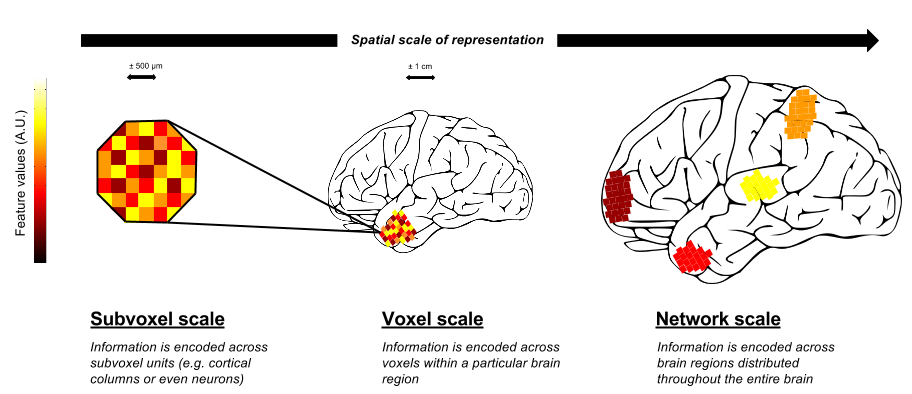
\includegraphics[width=\textwidth]{spatial_dist4}
\end{figure*}

A key question in neuroscience is how the brain \emph{represents} information at different scales of observation, with appropriate measurement and analysis tools for each scale. An important technique in the neuroscientist's toolbox is functional magnetic resonance imaging (fMRI). With fMRI, neuroscientists have been able to probe how the brain maps information onto informational units known as \emph{voxels}, cubic entities encompassing information about brain activity at the millimeter scale (usually 1-5 mm). While the technique's spatial resolution is, up to this day, unparalleled in in-vivo human neuroimaging, it still measures, at best, aggregated energy consumption of thousands of neurons. Despite the limitation of examining information representation at the sub-voxel level, fMRI research has proven its use in helping neuroscientists discover how the brain represents information at larger scales.

A traditional approach in cognitive neuroscience research is to investigate representations of psychological concepts and processes as significant activations or deactivations of parts of the brain using fMRI. This type of analysis is commonly referred to as ``univariate analysis'', because it assesses each unit of measurement (i.e. voxel) in the brain separately as independent univariate models \cite{friston1994}. Often, studies applying such whole-brain univariate analyses result in color-rendered brain-maps demonstrating significant (de)activations, leading researchers to conclude that the plotted regions are involved in the psychological concept or process under examination. Alternatively, researchers may summarize differences in mean activity levels across conditions for different regions which are selected based on an initial whole-brain univariate analysis.  

% Dit moet uitgebreider. Wat kan univariate analysis niet wat multivariate analyses wel kunnen?
However, while whole-brain univariate analyses are useful as a visualization tool to display involvement of single voxels, it does not allow for direct statistical tests of priori hypotheses about how the brain represents types of information or processes. For example, a whole-brain univariate analysis of the representation of emotional pictures may reveal that this concept is represented neurally as a set of distinct ``blobs'' across the brain (see e.g. \citeNP{lindquist2015}). Consequently, the researcher in question may conclude that emotions are represented as a global functional network including brain region \emph{X}, \emph{Y}, and \emph{Z}. The issue here is that this interpretation is a \emph{qualitative} interpretation; no statistical test has been performed that warrants a quantitative conclusion about the network-representation of emotions. Moreover, the observed network-representation may be heavily dependent on how stringent one has corrected for multiple comparisons (on which no consensus exists to date, \citeNP{woo2014}. It may well be that the observed network is reduced by a single cluster or smaller set of voxels when a more stringent correction method is adopted. % Steven zegt hier iets over "to test has been performed to exclude all other areas of the brain", maar daar ben ik het niet mee eens.
Thus, univariate analyses seem to suffer from issues that warrant straightforward interpretation of the results. 

One way to overcome the limitation of univariate analysis to test \emph{a priori} hypotheses \emph{quantitatively} is to model information as a multivariate pattern. This is exactly the approach of \emph{multivariate pattern analysis} (MVPA), a fairly recent analytical tool in neuroimaging that allows for investigation of neural representations as spatially distributed patterns of activation \cite{haxby2001,kriegeskorte2006}. By explicitly modelling neural representations as a set of informational units instead of each individual unit separately, multivariate analyses allow for direct tests of whether a small cluster of voxels, a brain region, or a network contains reliable information about the investigated representation, allowing for easy-to-interpret statistical tests.        

Currently, multivariate pattern analyses are widespread in almost all domains of cognitive, affective, and social neuroscience. For example, in vision research, MVPA has been applied to accurately decode stimulus orientation from subregions in V1 \cite{kamitani2005}. At a coarser scale, researchers have shown that it is possible to decode memory components in various distinct regions in the brain \cite{chadwick2010,visser2013}. More recently, MVPA has surfaced in the social and affective neuroscience literature, in which it has been used to investigate broadly distributed representations of social and emotional processes. For example, \citeA{kassam2013} has shown that MVPA can be used to decode representations of different emotions. 

MVPA thus seems to be applicable to investigate topics for various types of representational content. It is likely, however, that the scale at which representations are manifested in the brain differ depending on whether one investigates, for example, low-level stimulus features (such as spatial frequency or stimulus orientation) versus high-level cognitive or affective processes (such as decision-making or emotional experience). This notion of potential differences in the spatial scale of representations, however, appears not to be considered often in constructing multivariate models aiming to map representations onto the brain. More specifically, in what will be discussed next, many MVPA studies seem to assume that representations are encoded at a voxel-level scale within spatially restricted regions in the brain, regardless of the type (low-level vs. high-level) of representation that is investigated.    

\subsection{Spatial distribution of low-level and high-level representations}
\noindent In the early years of MVPA, the technique was mainly used in cognitive neuroscience studies investigating low-level psychological concepts such as the representation of basic stimulus features (e.g. orientation, color, and motion direction) and object category (e.g. investigating the differences in representation between faces and houses). These low-level representations are known to be represented in spatially-restricted, contiguous patches of cortex, such as the representation of low-level stimulus features in (extra)striate cortex \cite{kamitani2005,parkes2009} and the representation of object categories in ventral temporal cortex \cite{haxby2001,eger2008,rice2014}. With the application of MVPA to higher-level psychological concepts and processes, the assumption that representations are encoded locally seems to have remained largely unchanged. This assumption about spatial distribution is, however, inconsistent with the emerging perspective of high-level psychological concepts and processes as interdependent globally distributed brain networks \cite{bressler2010,barrett2013,bullmore2009}. Despite this, many MVPA studies on these higher-level topics have limited their analyses to spatially-restricted, contiguous subsets of the brain. 

One possible explanation for the tendency to restrict multivariate analyses to small, spatially-contiguous subsets of the brain is the need for stringent feature selection in multivariate analyses. Typical MVPA datasets usually suffer from what is known as the \emph{curse of dimensionality} \cite{haynes2015}, which can be understood in the context of multivariate analyses as having more features than observations \cite{mahmoudi2012}. Having more features than observations often leads to \emph{model overfitting}, which is characterized as low generalizability of one's multivariate model to independent data. MVPA datasets are generally characterized as having more features (i.e. voxels) than observations (i.e. trials or runs). With state-of-the-art MRI-scanners (which may image voxels at 1-3 cubic millimeters), patterns of functional activation may amount to 250,000 voxels per trial, while typical experiments contain often not more than 100 stimulus presentations per condition. To generate accurate and generalizable models, MVPA studies thus often need to perform a type of \emph{feature selection} in order to reduce the dimensionality of the data.

Commonly, feature selection methods reduce dimensionality by limiting the spatial extent at which representations are investigated, which essentially limit or even preclude the possibility of revealing globally distributed representations. For example, one prevalent MVPA technique, \emph{searchlight analysis} \cite{kriegeskorte2006}, maps representations by analyzing representations in small spherical clusters of voxels throughout the brain (see for example \citeNP{clithero2009,skerry2014}). Although it is theoretically possible to extend the radius of the sphere to accommodate larger clusters, in practice most searchlights contain not more than 100 voxels \cite{etzel2013}. Moreover, although searchlights are often applied across the entire brain to investigate the possibility of multiple \emph{independent} sites at which the representation is encoded, searchlight analysis does not allow to investigate representations as a \emph{dependent} set of spatially-segregated clusters. 

Another common technique that reduces features by limiting the spatial extent of neural representations is \emph{region-of-interest analysis} (ROI-analysis; \citeNP{norman2006}), in which the representational space is reduced to a single brain area (see for example \citeNP{chavez2015,harry2013}). Here, an example would be to investigate representations of negative versus neutral emotions solely in the amygdala (see e.g. \citeNP{martinez2014}). Like searchlight analyses, representations could be investigated across several regions-of-interest (by for example investigating the insula and orbitofrontal cortex in addition to only the amygdala), but, like searchlight analyses, this assumes that representations are independently encoded in these regions and do not allow to investigate whether representations are encoded in a set of dependent, spatially-segregated regions.

One way to reduce the effects of the curse of dimensionality and remain the possibility of revealing global representations is to adopt a fully data-driven feature selection on the entire set of voxels. A popular whole-brain feature selection method is to select only the voxels with the largest univariate differences across conditions (usually referred to as \emph{univariate feature selection}; \citeNP{mitchell2004}). In other words, per voxel, a two-sample independent t-test (or ANOVA in case of more than two conditions) is computed to investigate univariate condition differences and only voxels with a t-value or F-statistic above a certain threshold are selected (e.g. \citeNP{saarimaki2015}). Another whole-brain feature selection method is to select the most ``stable'' voxels across stimuli presentations of the same condition (see e.g. \citeNP{shinkareva2008,baucom2012}, which is operationalized as selecting voxels with the highest mean correlation among pairwise correlations across stimulus repetitions within the same experimental condition.           

A major advantage of these whole-brain feature selection methods is that they are, a priori, blind to spatial distribution of the selected voxels and therefore allow for investigation of globally distributed representations. This technique is therefore especially useful in analyzing widespread functional networks, which are often reported in (univariate) studies on higher-level cognitive processes (e.g. \citeNP{lindquist2015,barrett2013}). Recently, several MVPA studies on higher-level psychological concepts and processes have shown that, indeed, whole-brain feature selection yields representations consisting of several spatially-discontinuous clusters. \citeA{kassam2013}, for example, used whole-brain stability-driven feature selection to reveal a broadly distributed network involved in representation of discrete emotions, including regions from the frontal lobe (orbitofrontal cortex), temporal lobe (anterior temporal lobe), and parietal lobe (supramarginal gyrus). Similarly, studies on other high-level psychological concepts and processes, including example Theory of Mind \cite{corradi2014}, motivation \cite{etzel2015}, emotion regulation \cite{ochsner2002}, and emotional valence \cite{baucom2012}, reveal globally-distributed representations spanning the entire brain.

(Theoretically, instead of univariate feature selection, one could use multivariate feature selection methods, such as Recursive Feature Elimination \cite{demartino2008}, to select sets of voxels. However, doing this at a whole-brain level is computationally near impossible, as this would entail testing all possible combinations of 250,000 voxels. Therefore, this technique is most often used after other dimensionality techniques haven been applied, such as region-of-interest selection \cite{norman2006}. Moreover, dimension reduction techniques involving linear transformation of features into components, such as PCA, are other potential whole-brain feature selection methods, but are rarely used in fMRI research due limited interpretability of results and therefore not discussed here.)

In sum, in contrast to spatially-restricted feature selection methods such as ROI- and searchlight analyses, whole-brain feature selection allows for investigation of globally distributed representations, which are likely to be found when investigating high-level psychological concepts and processes. Given a globally distributed representation, the question remains how information is encoded within this globally distributed pattern. In many MVPA studies on low-level stimulus features, for example, it is assumed that representational information is encoded within a set of (largely) independent voxels. This voxel-level encoding of this type of low-level representations has been largely supported by neurobiological evidence that many stimulus features, such as spatial frequency \cite{tootell1981}, orientation \cite{yacoub2008}, and color \cite{hadjikhani1998}, are encoded (often retinotopically) at the level of cortical columns (which are about 0.5 mm in width). In other words, low-level stimulus features are believed to be encoded across features at the scale of voxels and investigating representations of such low-level stimulus features as patterns of voxel-level information is sensible. This largely implicit assumption of what could be described as \emph{voxel-level dimensionality} seems to have been taken over by MVPA studies on representations of high-level psychological concepts and processes. Contrary to most high-level MVPA studies, however, there are good reasons to believe that these high-level representations are encoded at a coarser scale than the voxel-level scale of low-level representations.

\subsection{Spatial scale of low-level and high-level representations}
\noindent The assumption that multivariate representations are encoded at the scale of voxels is likely due to early MVPA studies investigating low-level stimulus features that are known to be organized across cortical columns in visual cortex. Initially, decoding accuracy of such stimulus features were thought to arise from unequal distributions of feature values within voxels, which has led to the belief that MVPA may be sensitive to subvoxel (i.e. columnar) information \cite{haynes2005,kamitani2005}. Quickly following these studies suggesting subvoxel sensitivity, a study by \citeA{opdebeeck2010} contested this claim by showing that spatial smoothing, which effectively reduces spatial resolution of multivariate patterns, did not negatively affect accuracy of decoding features, which were presumed to be encoded at the subvoxel-level. This finding was later directly supported by another study \cite{freeman2011} that showed that, at least for the low-level feature of stimulus orientation, a relatively coarser feature map existed which appeared to be related to the radial bias of presented stimuli. These studies thus suggest that representations may contain information at multiple scales: at the (sub)voxel scale and a scale coarser than single voxels.

Several other studies have investigated this notion of multiple representational spatial scales using both simulations \cite{bulthe2014} and experimental research \cite{drucker2009,swisher2010,bulthe2015}. One notable study by \citeA{brants2011} provides a particularly compelling example how different types of representations may be encoded at different spatial scales by contrasting spatial scale of representations of object category and within-category examplars. As the identity of within-category examplars largely depend on low-level stimulus features \cite{eger2008,rice2014}, it was hypothesized that their respective neural patterns would be encoded on a smaller spatial scale relative to the patterns of object categories. Indeed, examining these two types of representations in the frequency domain indicated that object categories contained more power in lower (spatial) frequencies compared to within-category exemplars. Further supporting their hypothesis of ``multiscale'' functional representations, it was demonstrated that spatial smoothing improved representational distances between different object categories more than representational distances between within-category exemplars. Importantly, while most studies on multiscale representations have shown that particular low-level stimulus features are represented at different scales, the \citeA{brants2011} study provides support for the notion that low-level psychological concepts (e.g. stimulus features) are encoded at a finer scale than relatively more high-level concepts such as object-category. 

Another line of evidence for different spatial scales for low-level and high-level representations comes from the observation that many univariate studies (or whole-brain MVPA studies) on high-level concepts or processes yield global networks consisting of \emph{clusters} of voxels (e.g. \citeNP{oosterwijk2015,kassam2013,corradi2014,lindquist2015}). This spatial clustering is unlikely if individual voxels within these clusters carry unique information. This dependence between voxels within clusters has been further supported by the fact that spatial smoothing \cite{oosterwijk2015,kassam2013} does not affect information encoded within representations encoded across clusters. One study by \citeA{ethofer2009} even explicitly demonstrated that classification of representations of auditory emotional information, which was revealed to be represented in a set of globally distributed clusters, actually improved after spatial smoothing. These studies indicate that spatially-clustered voxels are highly correlated and thus individual voxels within clusters carry redundant information about the representation. Essentially, individual clusters in high-level representations likely do not contain multivariate information, but rather univariate information encoded as average activity within the cluster. Consequently, high-level representations are likely encoded as a multivariate network of clusters (corresponding to the \emph{Network scale} in Figure 1). 
In sum, the literature on multivariate representations of psychological concepts and processes suggest that there is a distinction at which representations are fundamentally \emph{organized} and how they are ordinarily \emph{analyzed}. While there is evidence for (sub)voxel-level dimensionality of low-level representations and larger-scale network-level dimensionality of high-level representations, many studies on high-level psychological concepts and processes analyze the respective globally distributed patterns at the voxel-level, treating individual voxels as independent informational units. This question about the spatial scale of independent features within global representations forms this study's main research question. In attempting to answer this question, the current study may contribute to fundamental theoretical understanding of the concept of neural representation by investigating the dimensionality of high-level representations. In turn, improved understanding of the structure of high-level representational data may lead to optimization of multivariate techniques by, for example, employing cluster-thresholding methods on the initial feature selection, as is done in the current study. Lastly, if shown that high-level representations are indeed encoded at a coarser scale than the voxel-level, multivariate analyses can be substantially sped up by reducing the redundancy in the amount of parameters of multivariate models of fMRI representations.

\subsection{Current study}
\noindent To investigate the dimensionality of global representations, this study reanalyses the data from a previous study (\citeNP{oosterwijk2015}; see appendix A for a justification of the deviation from the original proposed experiment). In this study, we examined the neural overlap between components of self-experienced emotions and understanding emotions in others using multivariate pattern analysis with a linear support vector machine classifier \cite{chang2011}. Here, we reanalyse the data from only the self-experienced emotion patterns, because this data yielded the largest effect size (60\% classification accuracy at 33.3\% chance level) and the most robust global representation in which spatial clustering of features following univariate feature selection was clearly visible (see figure 2). Note that the observed global representation in the \citeNP{oosterwijk2015} study appears to correspond to global representations of emotion networks in several other MVPA studies \cite{kassam2013,saarimaki2015,kragel2015} and univariate studies (see for a meta-analysis \citeNP{lindquist2015}).

\begin{figure*}[ht]
\floatfoot{\textbf{Figure 2}: Global representation of self-experienced emotion components in the \citeA{oosterwijk2015} study. The representation reflects the univariate feature selection as normalized difference scores across conditions averaged over iterations and subjects. Difference scores are computed as the average pairwise differences between the mean patterns of conditions, normalized across voxels. The global representation contains several spatially-segregated clusters, including clusters in the anterior temporal lobe, lateral occipital complex, supramarginal gyrus/angular gyrus (temporal-parietal junction), inferior frontal gyrus, frontal pole (dorsolateral prefrontal cortex), and central opercular cortex.} 
\centering
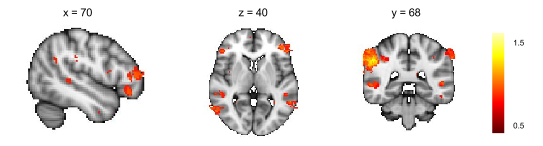
\includegraphics[width=\textwidth,height=5cm]{UnivariateFeatureSelection}
\end{figure*}

Given the apparent spatial dependence between voxels in correlated clusters, we hypothesize that, instead of multivariate patterns across voxels, global representations are encoded as a pattern of cluster-wide features. If this is indeed the case, a multivariate set of averaged clusters should contain the same representational information as the same data in which no within-cluster averaging has been performed. To investigate this hypothesis, we analyzed the data in two different ways. First, as a benchmark, we performed univariate feature selection before classification (similar to the original Oosterwijk et al. study), effectively disregarding the possible lower dimensionality of the data (``benchmark analysis''). Second, to directly test whether a set of clusters, instead of voxels, underlies the investigated representations, we perform a cluster-thresholding procedure on the selection of voxels yielded by an initial univariate feature selection (similarly to \citeNP{michel2012}). Clusters resulting from this cluster-thresholding procedure are subsequently averaged and used as features in the classification analysis (``cluster-average analysis''; see figure 3 for a graphical representation of the two contrasted analyses). 

We expect that, if representational information is indeed encoded across spatially-correlated clusters, classification accuracy of the cluster-average analysis will not be significantly lower than in the benchmark analysis. Moreover, we expect that the average feature correlation, calculated as the mean pairwise correlation across trial-vectors of each feature, is lower in the cluster-average analysis compared to the benchmark-analysis, as the former analysis should reduce the redundancy in features by spatial averaging. 

\begin{figure*}[ht]
\floatfoot{\textbf{Figure 3}: Graphical representation of the two performed analyses. The benchmark analysis (upper diagram) uses all voxels which are returned from a univariate feature selection procedure as features in the classifier. The ``cluster-average analysis'' performs a cluster-thresholding procedure on the features yielded by an initial univariate feature selection and subsequently uses the within-cluster averages as features.} 
\centering
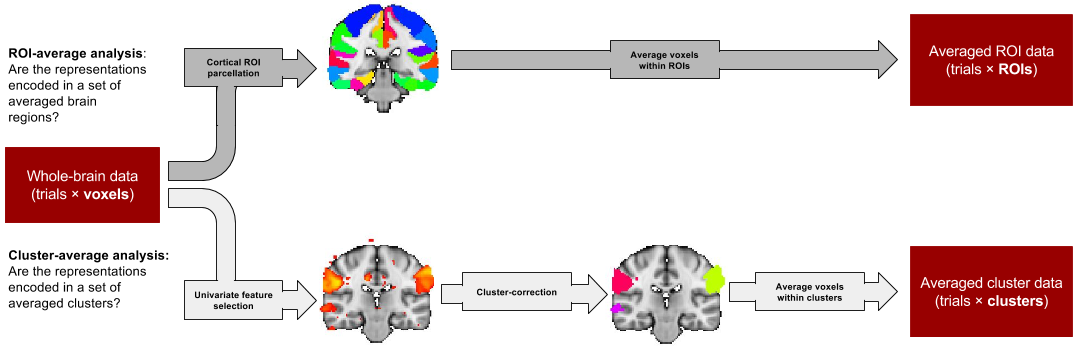
\includegraphics[width=\textwidth,height=8.5cm]{methods}
\end{figure*}

\section{\Large \textsc{Methods}}

\subsection{Dataset}
\noindent The dataset used for this research is from the \citeA{oosterwijk2015} study. The goal of this study was to examine the neural overlap between representations of \emph{self}-focused emotional experience and representations of processes involved in understanding emotions of \emph{others}. Specifically, the study hypothesized that the same basic psychological processes -- representations of (1) sensorimotor, (2) interoceptive, and (3) situational information -- underlie both emotion experience in the self and emotion understanding of others. Using a multivariate classifier, it was shown that the representations of these three components in the self-condition could be reliably decoded from their respective neural patterns and, importantly, that these neural representations of self-focused emotion components could be used to differentiate the corresponding components involved in emotion understanding of others significantly above chance (for a more nuanced interpretation of the results, see the original article).

This study only reanalyses data from the self-focused emotional imagery task. In total, thirteen subjects completed two identical runs of this task. One subject was excluded due to incomplete data. The stimuli consisted of short linguistic cues describing either emotional actions or expressions (representing the sensorimotor component; n = 20), bodily feelings (representing the interoception component; n = 20), or situations (representing the situational component; n = 20). Examples would be, for example, ``To make a fist'', ``To have a racing heart'', and ``Your house is on fire'', respectively. Participants were asked to imagine these actions/expressions, bodily feelings, and situations as if they were experiencing those themselves. The stimuli (120 in total; 20 per condition across two identical runs) were presented in a fully event-related design for six seconds each with a fixed inter-stimulus-interval of two seconds. Functional BOLD-MRI data was acquired with a 3T Philips Achieva MRI-scanner, using echo-planar-imaging with a TR of 2000 ms and a TS of 27.63, imaging the entire brain volume using 37 slices (yielding a voxel size of 3 $\times$ 3 $\times$ 3 mm, with a slice gap of 0.3 mm; for more details on the experimental materials, design, and fMRI acquisition parameters, see \citeNP{oosterwijk2015}).

\subsection{Preprocessing and first-level analysis}
\noindent The functional data from the two runs were preprocessed using various FSL functions. Preprocessing steps included slice-time correction, motion correction, spatial smoothing (FMWH: 5 mm), temporal filtering (Savitsky-Golay filter), and registration to subject-specific anatomical T1 images and subsequently to standard MNI152 (2mm) space using a non-linear transform. Resulting preprocessed time series were subjected to a first-level GLM analysis. Single-trial regressors were created by convolving trial-specific stimulus onsets with a canonical HRF, modelled using a double gamma function. Beta-coefficients yielded by the GLM were normalized by the regression's mean squared error, effectively yielding whole-brain patterns of t-values per trial. After masking these patterns by a gray matter mask (excluding white matter and CSF voxels) derived from the Harvard-Oxford probabilistic cortical atlas in FSL (without a minimum probabilistic threshold), subject-specific matrices of trials (120) $\times$ voxels (269412) were created to be used in the classification analysis. These trial $\times$ voxel patterns were additionally scaled using a standard z-transform (zero mean, unit variance) across voxels. 

\subsection{Classification analysis}
\noindent The two analyses (the benchmark and cluster-average analysis) were kept as similar as possible to avoid differences in classification score attributable to other factors than the methodological manipulation of the analysis' features. The parameters held constant included all preprocessing parameters (i.e. spatial smoothing kernel, low-pass filter, initial brain mask, scaling) and parameters specific to classification analyses (i.e. choice of classifier and the amount of test-trials). The values of these parameters used in this study's analyses were determined through a cross-validated parameter-optimization procedure in the Oosterwijk et al. study based on recommendations outlined by \citeA{kay2008} and \citeA{kriegeskorte2009}. See the original study by Oosterwijk et al. for more information. Following this optimization-process, a smoothing kernel of 5 mm, no low-pass filter, a whole-brain gray matter mask, standard z-transformation (zero-mean, unit variance) for feature scaling, four-test trials per condition per iteration, and a linear support vector machine classifier were chosen to apply on the remaining validation dataset.

Furthermore, as we use a repeated random subsampling procedure (known as a ``stratified shuffle split'' in the Python scikit-learn environment), a fixed random seed (random\_state = 0) was chosen for the following analyses to avoid subtle differences in results across analyses due to random sampling artifacts. For the linear support vector machine algorithm, the SVC function from the \emph{svm} module in Scikit-learn Python package was used. While potentially suboptimal, the algorithm's hyperparameter \emph{C} was not optimized (and thus set at its default value 1) to reduce computation time. Both the benchmark and the cluster-average analysis were iterated 100,000 times. The reported classification scores are expressed as the classification's \emph{accuracy} (averaged over subjects), which is calculated as:

\[\frac{\sum\text{True positives}+\sum\text{True negatives}}{\sum\text{Predictions}}\]

The classification-pipeline was implemented within the scientific Python environment, using primarily \emph{Numpy} (scientific computing package; \citeNP{van2011}), \emph{Scikit-learn} (machine learning package; \citeNP{pedregosa2011}) for its classification algorithms and cross-validation tools, and \emph{pandas} (data analysis package; \citeNP{mckinney2012}) to summarize, analyze, and visualize results.

\subsection{Code availability}
\noindent The code for this study was version-controlled using git and stored in a publicly accessible online Github repository (\url{https://github.com/lukassnoek/MSc_thesis}). The majority of the code is contained in the modules \texttt{glm2mvpa.py} (containing functions to transform first-level single-trial contrasts to trial $\times$ feature matrices) and \texttt{main\_classify.py} (containing code for the classification pipeline; both are available from the Analysis\_scripts/Modules subdirectory in the Github repository). Code for plotting the figures contained in this report can be found in several IPython Notebooks in the Analysis\_scripts/Notebooks subdirectory. 

\section{\Large \textsc{Confirmatory results}}

\subsection{Benchmark analysis}
\noindent As a benchmark analysis, a classification analysis with the same parameters as the \citeA{oosterwijk2015} study was performed. Due to the switch from analysis environment in MATLAB to a Python environment (including switching from a LIBSVM implementation to Python's SVC classifier), reported results in this benchmark analysis may differ slightly from the results reported in the original study. 

\subsubsection{Analysis set-up and parameters}
\noindent The benchmark analysis uses a whole-brain univariate feature selection method. This method selects, in a univariate fashion, the most differentiating voxels from the entire set of voxels. To calculate a vector with the differentiation scores of voxels, the average normalized Euclidian distance across mean patterns (i.e. voxels averaged within conditions) is calculated. Thus, for \emph{K} conditions (i.e. classes in machine learning terminology), the differentiation score (\emph{ds}) for voxel \emph{x} is:

\[ \text{ds}(x) = \frac{1}{K(K-1)} \sum_{i,j=1}^{K}\left | x_{i}-x_{j}\right | \]

\noindent in which the distances are calculated between condition-average values. 

Given the results from the parameter optimization-procedure from the original Oosterwijk et al. study, the benchmark analysis used a differentiation score lower-bound of 2.3 (corresponding to a right-tailed p-value of 0.01 in a normal distribution, assuming that the differentiation scores conform to a Gaussian distribution).

\subsubsection{Benchmark results}
\noindent The benchmark analysis was able to correctly classify a significant proportion of the trials correctly, as evidenced by a one-sample t-test the classifier's mean accuracy (\emph{M} = 0.60, \emph{SD = 0.13}) given the null-hypothesis of chance-level classification (0.333), \emph{t}(11) = 7.089, \emph{p} < 0.0001 (see figure 4 for individual results). The average amount of voxels included in the classifier was 1042 voxels, which varied substantially between subjects (\emph{SD}: 593). Note here that the amount of features (on average 1042) surpasses the amount of observations (120 trials) by far. The fact that the model does not overfit to the extent of classification at chance-level suggests that the features are strongly correlated and, thus, that the dimensionality of the investigated representations is far lower than the amount of voxels yielded by an univariate feature selection procedure. Indeed, examining the average correlation across features reveals a significant average correlation of .37, \emph{t}(11) = 7.066, p < 0.0001. Interestingly, the height of correlation across voxel patterns seems to predict classification accuracy (\emph{r} = 0.54), albeit insignificantly ({\emph{p} = 0.07).     

\begin{figure}[ht]
\floatfoot{\textbf{Figure 4}: Results from the benchmark analysis. The bars represent the classification accuracy per subject; the dotted line represents accuracy at chance level (i.e. 0.333).} 
\centering
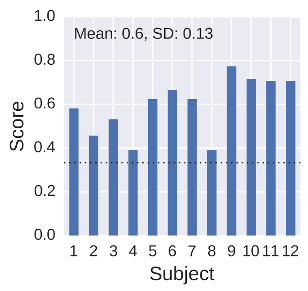
\includegraphics[width=\textwidth]{benchmark_plot}
\end{figure}

% Misschien hier brain-plotje?
\subsection{Cluster-average analysis}
\noindent The cluster-average analysis is performed to investigate whether the dimensionality reduction by averaging features within observed clusters in the data following univariate feature selection does not significantly affect classification accuracy relative to the benchmark analysis.

\begin{figure*}[ht]
\floatfoot{\textbf{Figure 5}: Results from the grid search optimization of minimum cluster size and differentiation score parameter values. Cells with scores below chance level (0.333) are set to 0 to improve color contrast in the remaining cells. The boxed cell in the grid indicates the highest classification accuracy (0.571).} 
\centering
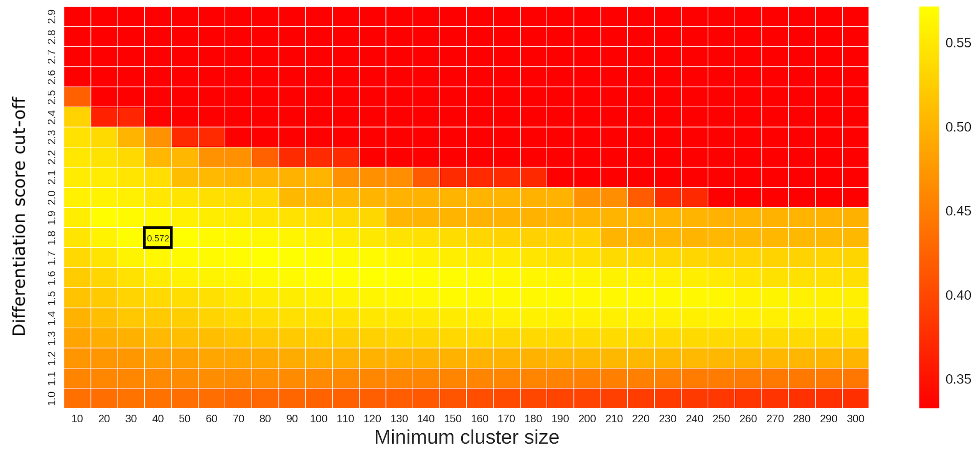
\includegraphics[width=\textwidth]{gridsearch_clustercorrect}
\end{figure*}

\subsubsection{Analysis set-up and parameters}
\noindent In the cluster-average analysis, an additional cluster-thresholding and averaging step is added after regular univariate feature selection is performed in the benchmark analysis. After univariate feature selection using a given a differentiation score cutoff, simple cluster-thresholding is applied to the feature set with a minimum cluster size parameter indicating the minimum amount of spatially contiguous voxels that should be contained in a cluster. FSL's clustering algorithm was used to identify clusters within the set of voxels yielded by the univariate feature selection (\url{http://fsl.fmrib.ox.ac.uk/fsl/fslwiki/Cluster}). After cluster-thresholding, features within spatially segregated clusters are averaged and subsequently used as new features in the classification analysis (i.e. yielding a trails $\times$ cluster array).  

Effectiveness of this cluster-thresholding method likely depends strongly on the combination of the minimum differentiation score and minimum cluster size, as lower differentiation scores will yield larger clusters and the other way around. To empirically determine the most optimal settings for these parameters, the cluster-average classification analysis was run for all different combinations of minimum cluster size (ranging from 10 to 300 voxels in steps of 10) and minimum differentiation score (ranging from 1 to 3 in steps of 0.1). This process, akin to an exhaustive grid search optimization procedure, was run with 250 iterations for each analysis. 

Results from the grid search procedure indicated that a minimum cluster size of 40 voxels in combination with a minimum differentiation score of 1.8 yields the highest classification accuracy (i.e. 0.572; all results are plotted as a heatmap in figure 5). This result, however, should be interpreted with care. First, as apparent from figure 5, near-optimal classification scores can be achieved by a wide range of different combinations of the two cluster parameters. By visual inspection, it appears that classification accuracy remains stable with minimum differentiation scores ranging from 2.1 to 1.5, as long as lower differentiation scores are combined with higher thresholds for minimum cluster size. This observation suggests that lower differentiation scores allow to capture larger clusters, which should be enforced by higher thresholds for minimum cluster size to exclude inclusion of spurious voxels which are not likely to occur in large clusters (assuming that the investigated representation is truly encoded across large clusters of voxels). Furthermore, this grid search procedure was performed on the same data on which the actual cluster-average analysis was performed, which implies double-dipping. Although in this case double-dipping refers to the model's hyperparameters (and not the model's actual parameters), still the risk of overfitting should be taken into account in interpreting these particular results and especially their generalizability.  

\begin{figure*}[ht]
\floatfoot{\textbf{Figure 6}: Results from the cluster-average analysis. The left panel displays classification accuracy per subject; the dotted line indicates accuracy at chance level. The right panel shows the correlation between accuracy scores in the benchmark and cluster-average analysis.} 
\centering
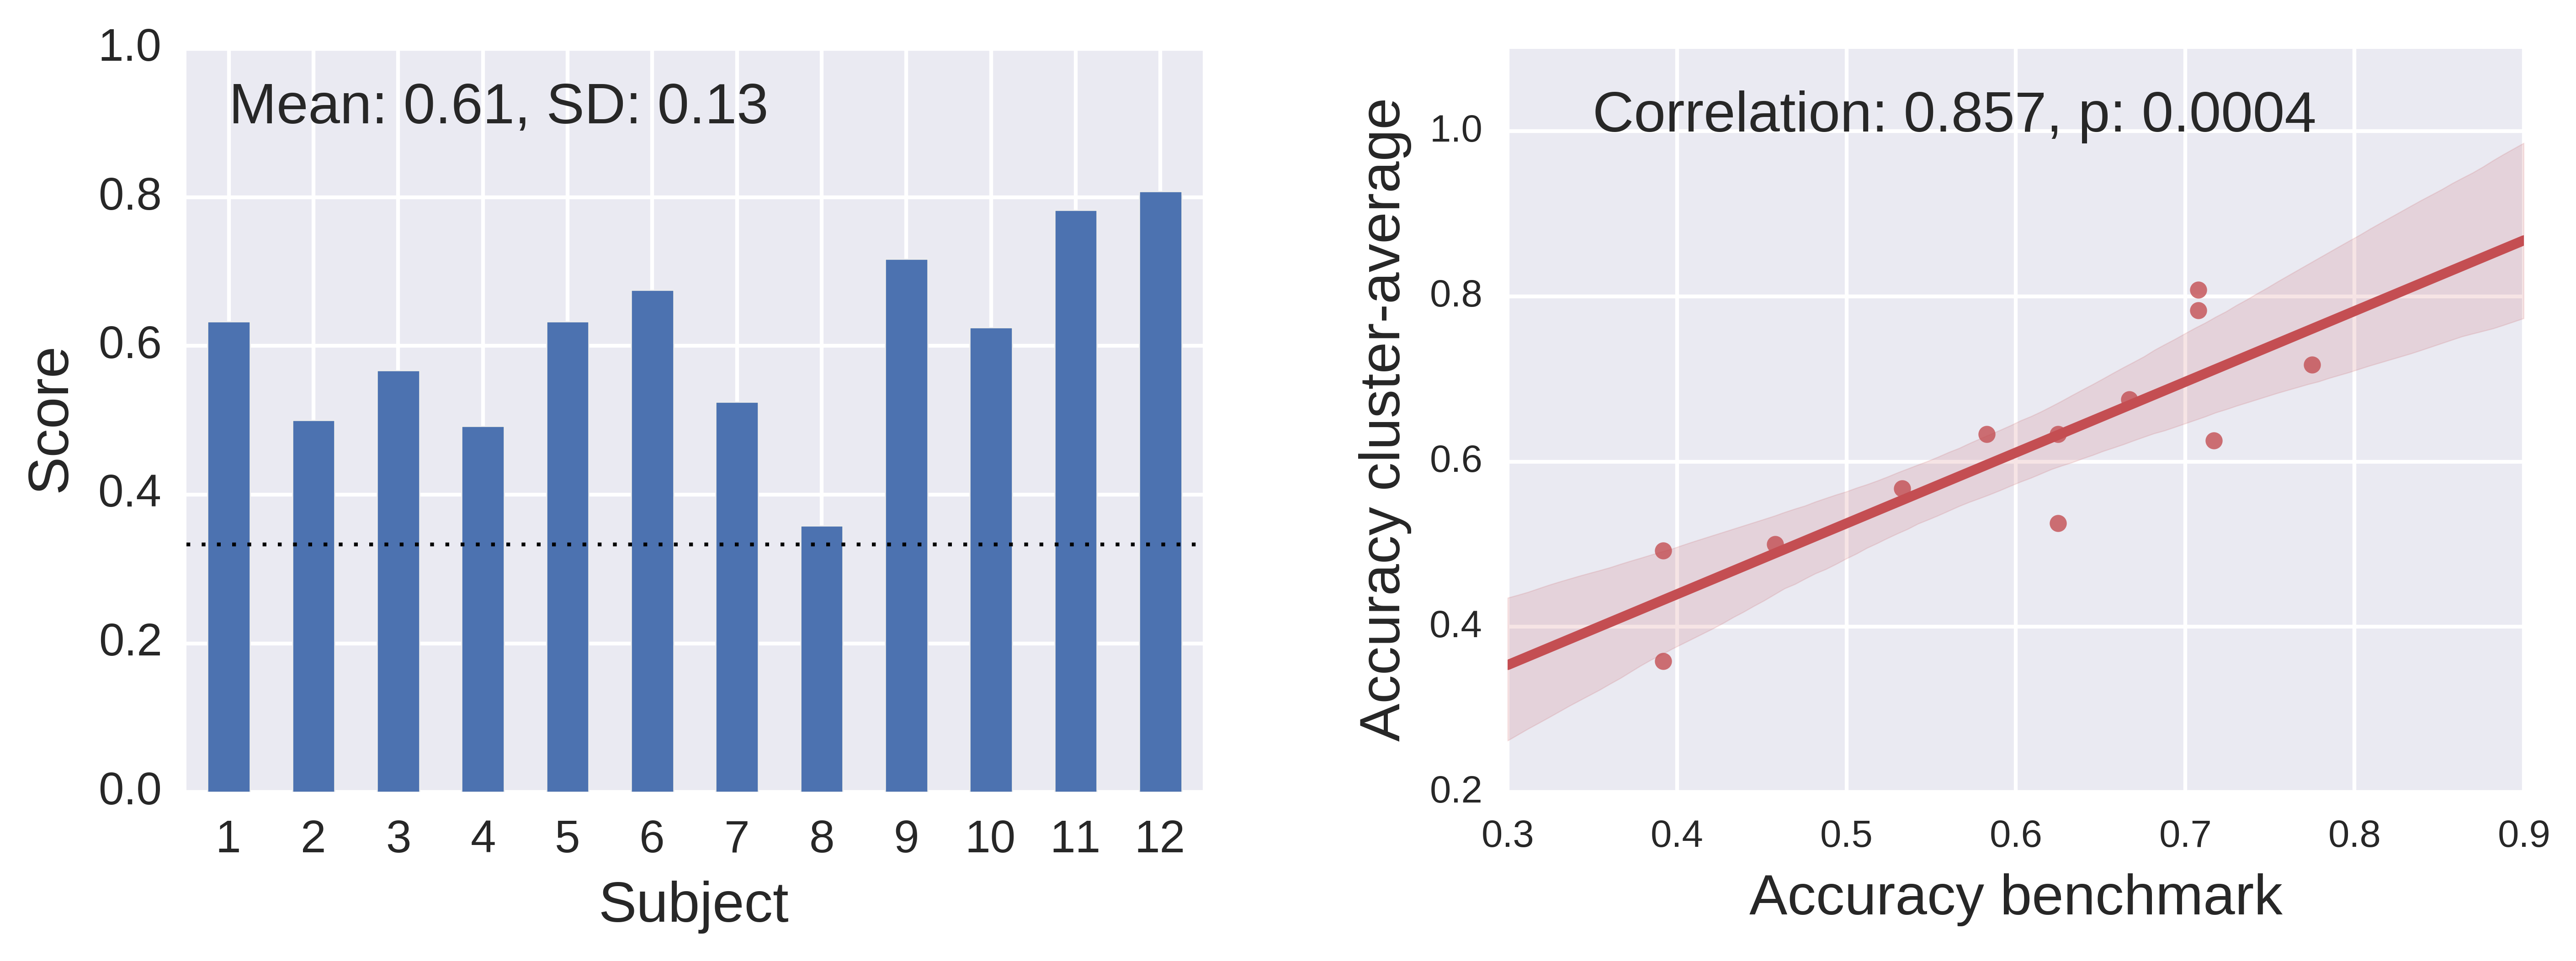
\includegraphics[width=\textwidth]{Cluster_average_plot_new}
\end{figure*}

\subsubsection{Cluster-average results}
\noindent As hypothesized, the cluster-average analysis was able to classify significantly above chance across subjects with a mean accuracy of 0.61 (\emph{SD} = 0.14), \emph{t}(11) = 7.388, \emph{p} < 0.0001 (see figure 6, left panel, for individual classification accuracies). Classification accuracy did, as predicted, not differ significantly from the benchmark analysis (\emph{p} = 0.595). Compared to the benchmark analysis, the average amount of features (\emph{M} = 27.14, \emph{SD} = 4.07) has been reduced by about 97\%, while yielding a comparable average classification accuracy. As a control analysis, the correlation between individual classification accuracies in the benchmark and cluster-average analysis was computed, which turned out highly significant (\emph{r} = 0.857, \emph{p} = 0.0004; see figure 6, right panel). This positive correlation suggests that, indeed, the cluster-average analysis capitalizes on the same information in the benchmark analysis, yet in a lower dimensional feature space. 

In contrast to this study's hypothesis, the average correlation between features in the cluster-average analysis (\emph{M} = 0.26, \emph{SD} = 0.08) was not found to be significantly lower than the correlation between features in the benchmark analysis (\emph{M} = 0.37, \emph{SD} = 0.16; \emph{p(difference)}} = 0.088).   

\subsection{Interim discussion and conclusions}
\noindent Thus far, this study's hypotheses regarding the dimensionality of high-level representations have largely been confirmed by showing that the cluster-average analysis yields comparable classification accuracy to the benchmark analysis while the amount of features was reduced by about 97\% compared to the benchmark analysis. 

The hypothesized reduction in mean feature correlation is, however, not fully supported by the results (see figure 7, lower left diagram), as the average feature correlation does not differ significantly between the benchmark and cluster-average analysis. One possible interpretation of this result is that spatial averaging in the cluster-average analysis might enhance the effect of structured noise. This type of noise may be represented at the scale of the analysis' clusters, such as the presence of draining veins or physiological resources (e.g. respiration or cardiac effects; \citeNP{birn2006}). Therefore, while the ``signal'' correlation between features may be reduced within the cluster-average analysis relative to the benchmark analysis, the measured ``aggregate'' feature correlation may be driven mainly by ``noise''-related components which may have been enhanced due to spatial averaging. 

In sum, cluster-average analysis has shown that the investigated global representations appear to be encoded as multivariate sets of clusters. In other words, multivariate information within ROIs or clusters seem to be redundant, as spatial averaging within ROIs or clusters does not affect classifier accuracy. However, it should be noted that classification problems within neuroimaging, such as predicting class labels based on fMRI data, is often severely ill-posed, meaning that multiple equally-valid solutions (i.e. multivariate models) may exist for a single problem (i.e. finding a particular classification score). Consequently, while we have shown that a model based on spatially-averaged, globally distributed features classifies accurately, the possibility of truly multidimensional voxel-level information within brain regions \emph{on top of a cluster-wide univariate effect} remains. Therefore, we conducted additional exploratory analyses in which we investigated classification with locally de-meaned patterns and, in addition, classification within ROIs separately.  

\begin{figure*}[ht]
\floatfoot{\textbf{Figure 7}: Comparison of accuracy (upper left plot), feature correlation (lower left plot), and number of features (right plot) between the benchmark and cluster-average analysis. All plots depict non-signficant differences at $\alpha$ = 0.01.} 
\centering
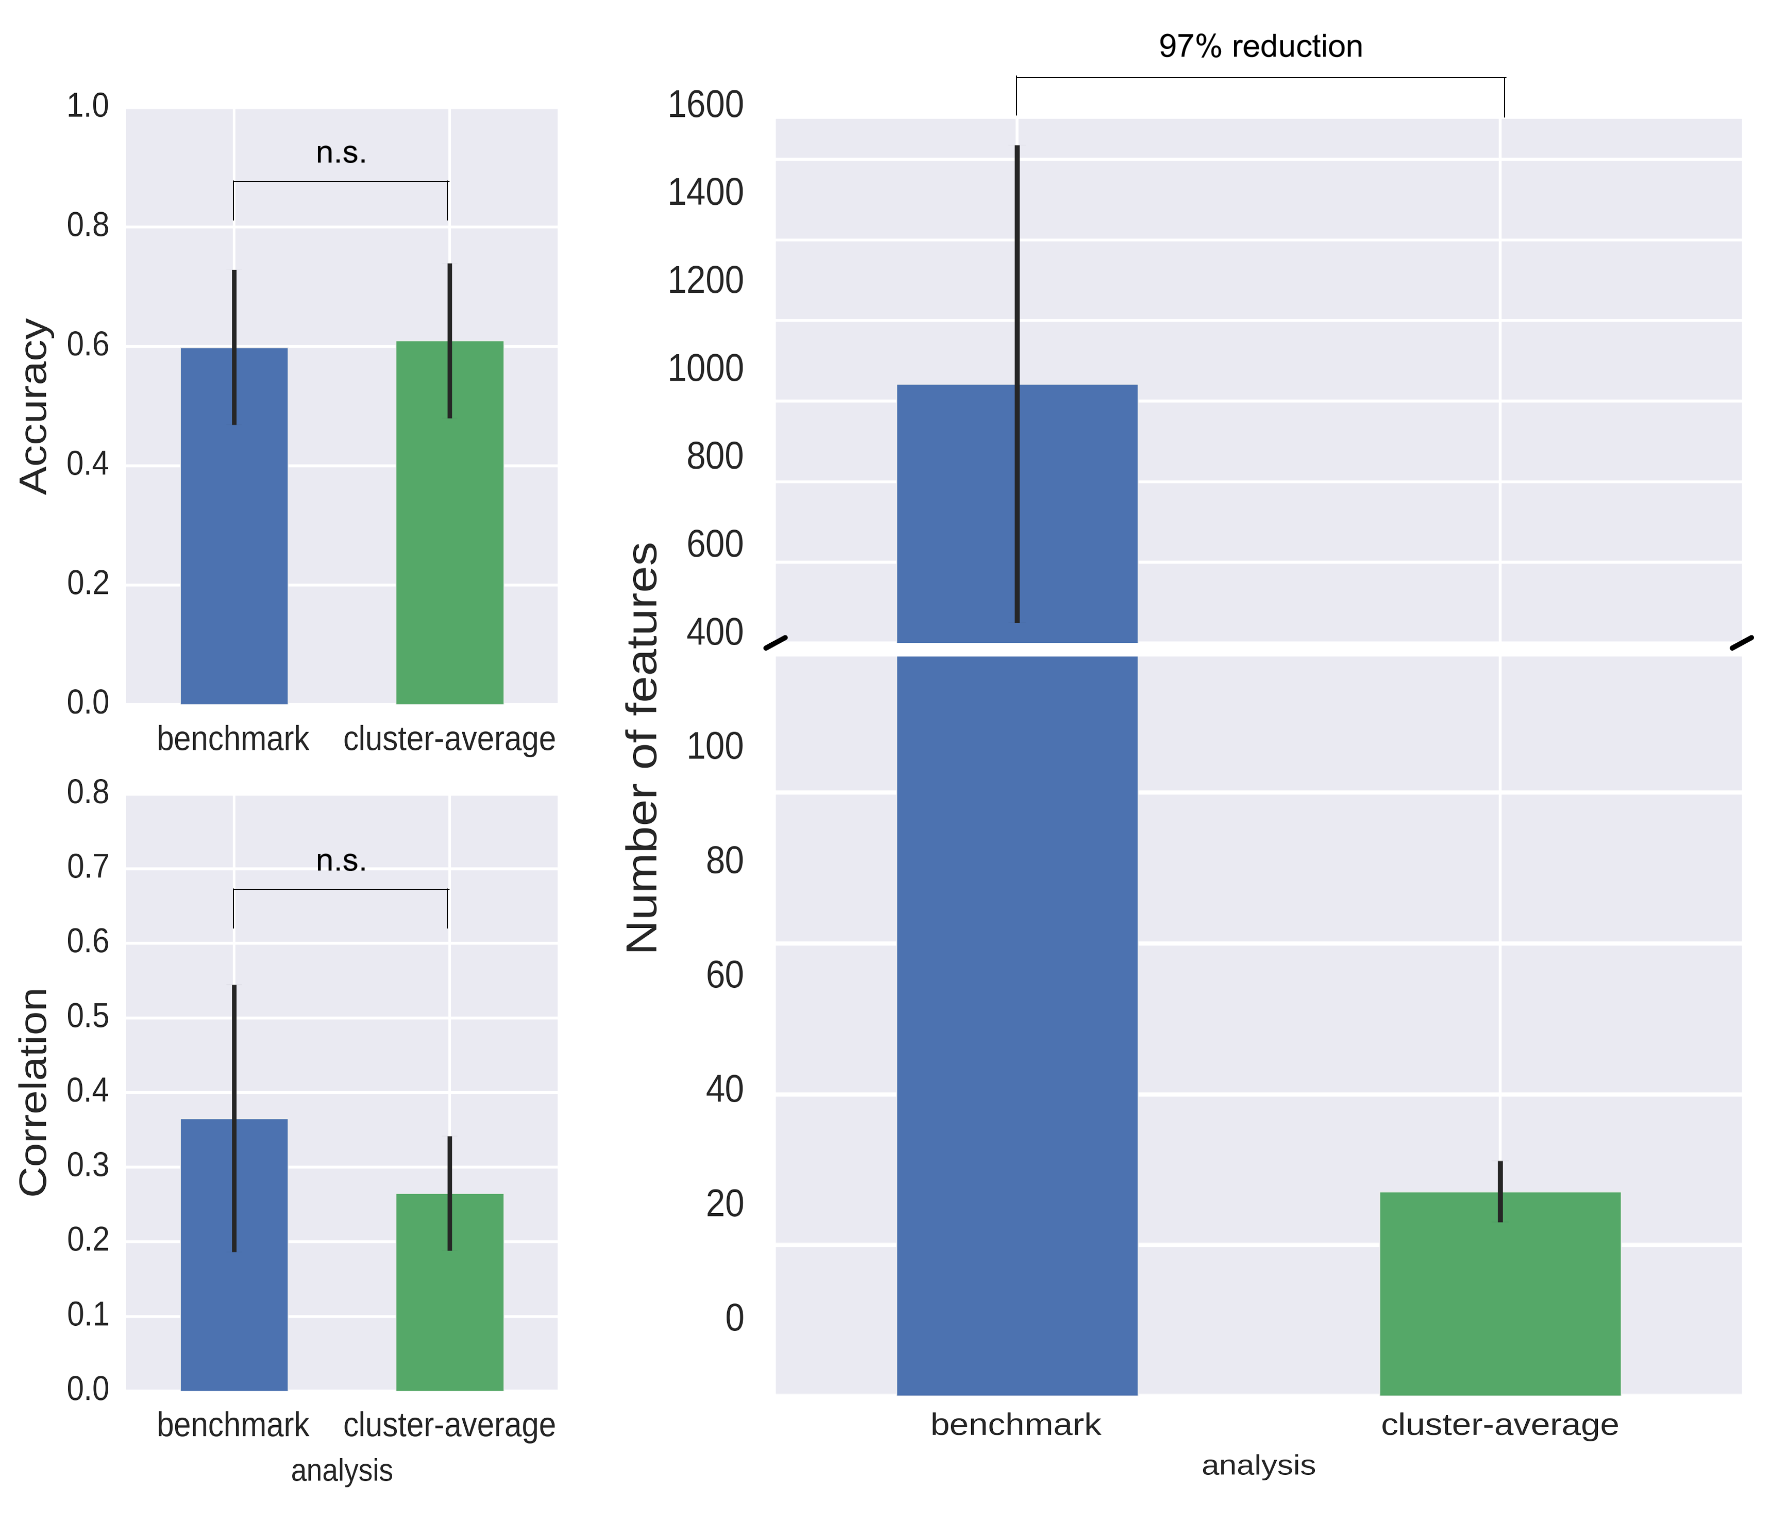
\includegraphics[width=\textwidth]{overview_plot}
\end{figure*}

\section{\Large \textsc{Exploratory results}}

\subsection{Classification with demeaned patterns}
\noindent This study's confirmatory analyses suggest that a set of averaged clusters encompass the true dimensionality of the investigated representations. In other words, univariate differences clusters, rather than fine-grained multivariate patters at the voxel-level, seem to drive classification of representations of global functional networks. Often, MVPA studies aim to demonstrate the exact opposite, i.e. that their investigated representations can be decoded through differences in their distributed multivariate pattern in \emph{absence} of any univariate influences \cite{davis2013}. One strategy to filter out possible univariate confounds is to subtract the mean activity from the each feature contained in the representation (see e.g. \citeNP{chikazoe2014,jimura2012,haxby2001}). If classification accuracy of demeaned patterns remains intact, it is often argued that the representation is truly multivariate \cite{davis2013,davis2014}. This demeaning strategy to prove multivariate encoding of representations has been explicitly advised in at least two methodological MVPA articles \cite{coutanche2013,kriegeskorte2006}. 

\subsubsection{Analysis set-up and parameters}
\noindent As an exploratory addition to the main analyses, representations in the cluster-average analysis are locally (i.e. within clusters) demeaned to investigate whether the representations are indeed driven by univariate differences between representations. As this study demonstrated that representations are encoded as univariate information within clusters, we subtracted each cluster's average value from each individual value within the cluster in both the train- and test-partition, effectively removing the influence of a cluster-wide univariate information. The resulting set of voxels across different clusters is subsequently used as features for the classification analysis. Consequently, as univariate information has been filtered out by demeaning, we expect that classification accuracy will drop to chance level.

\subsubsection{Demeaning results and discussion}
\noindent Surprisingly, classification accuracy was not degraded after demeaning the set of clusters (\emph{M} = 0.604, \emph{SD} = 0.14). This result can be interpreted in two ways. First, one may conclude that the investigated representations contain multidimensional information on top of univariate information, as is often concluded from accuracy classification following this demeaning strategy. Some evidence for an alternative possibility comes from a recent simulation study by \citeA{davis2014}, who showed that MVPA is sensitive to differences in voxel-level variance between patterns of different classes. In their simulations, they found that if one class was consistently associated with higher voxel-level variance compared to another class, the two classes could be accurately distinguished from each other using correlation-based and linear classifiers. Importantly, this effect holds \emph{in the absence of mean-pattern information}. 

\begin{figure*}[ht]
\floatfoot{\textbf{Figure 8}: Visualization of the demeaning procedure. First a univariate feature selection is performed, of which the resulting features are cluster-thresholded. Next, each individual cluster is demeaned across voxels and on the resulting patterns, a second iteration of univariate feature selection is performed, which yields presumably subclusters which ``survive'' the demeaning procedure.} 
\centering
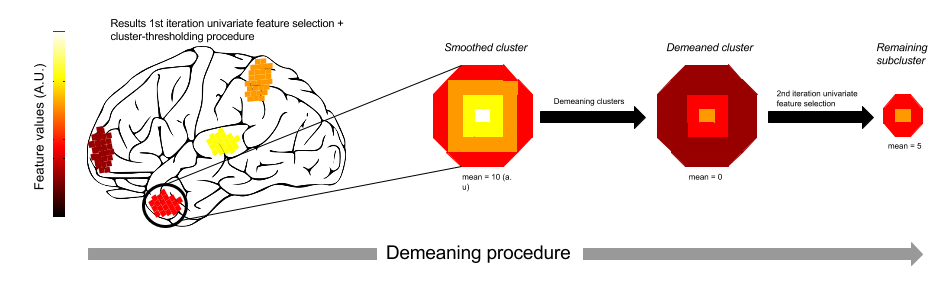
\includegraphics[width=\textwidth]{demeaning_clusters}
\end{figure*}

The findings from the \citeA{davis2014} study might, in turn, explain why demeaning does not effectively remove univariate influences within clusters in our study. When observing the not-cluster-thresholded data in figure 2 (from a classification analysis with a generic univariate feature selection), it appears that the spatial clustering of selected voxels is somewhat spatially smoothed: values at the edge seem to be lower than in the (geometric) centre of the cluster. Then, for example, trials from class \emph{A} could be distinguished from class \emph{B} if the former's representation would contain such a smoothed cluster and the latter's representation would not (i.e. would consist of merely white noise). Thus, one may conclude that the difference between class \emph{A} and \emph{B} consists of the presence of univariate information (i.e. a smoothed cluster). However, demeaning such smoothed clusters may not effectively remove univariate influences because it may be still contained as smaller clusters centered around the peak value of the original smoothed cluster. Put differently, demeaning may preserve univariate influences present at a smaller scale than at which the demeaning procedure was performed on. Then, while both patterns of class \emph{A} and class \emph{B} contain a mean of zero, differentiation between these patterns may be driven by subcluster univariate information present in class \emph{A} (which contained the original smoothed cluster) which is not present in class \emph{B}. 

\begin{figure*}[ht]
\floatfoot{\textbf{Figure 9}: Visual representation of classification accuracy yielded by within-ROI classification analyses. The plotted values represent t-statistics from a one-sample t-test of classification accuracy against chance level accuracy (0.333).} 
\centering
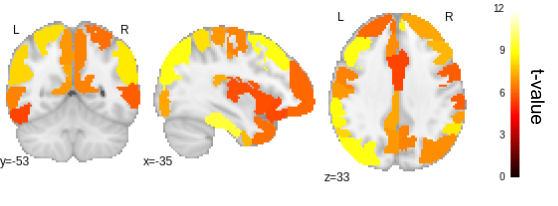
\includegraphics[width=\textwidth]{tmap}
\end{figure*}

To demonstrate residual univariate information in demeaned clusters, we performed a modified version of the demeaned cluster-average analysis as described in this section. After demeaning the clusters, we performed a second univariate feature selection, which was again cluster-corrected and averaged (see figure 8 for a schematic representation of this demeaning process). By averaging the features returned from the second cluster-thresholding procedure, we make sure that we capture univariate information. If there is residual univariate information left, we should be able to classify after a second iteration of cluster-thresholding and averaging. Indeed, this two-step cluster-average analysis with demeaned clusters demonstrates classification accuracy comparable to the original cluster-average analysis (\emph{M} = 0.54, \emph{SD} = 0.14). A two-sample t-test confirmed that the demeaning procedure did not yield a significantly lower classification accuracy, \emph{t}(10) = 1.27, \emph{p} = 0.11. This analysis shows that demeaned clusters contain residual univariate information that is likely encoded at a subcluster scale, suggested by the apparent spatial smoothing of clusters in the data. 

\subsection{Classification within separate ROIs}
Thus far, only global multivariate patterns have been investigated. While we have shown that a set of globally distributed averaged brain regions is \emph{sufficient} to distinguish high-level representations, this does not mean that this specific feature set is \emph{necessary} to distinguish these representations. As has been shown for low-level concepts such as visual stimulus properties \cite{swisher2010,drucker2009,freeman2011} and object category (\citeNP{opdebeeck2010,brants2011}; see also \citeNP{bulthe2015}), psychological concepts and stimuli may be represented at more than one spatial scale, again demonstrating that classification analyses attempting to answer questions about neural representation are often ill-posed. Because of this consideration of multiscale representations, we performed our benchmark classification analysis on various ROIs separately. Moreover, to investigate whether univariate information drives classification results, we perform the same analysis but with only the mean activity in each ROI instead of its multidimensional pattern. 

\subsubsection{Analysis set-up and parameters}
A total of 110 ROIs were drawn from the whole-brain Harvard-Oxford lateralized probabilistic cortical atlas. The minimum probabilistic threshold was set at 0, as this was also done for the initial whole-brain gray matter mask in the benchmark and cluster-average analyses. Note that this may cause substantial overlap of features between neighbouring ROIs. The classification analysis was performed on the patterns within each ROI separately. To speed up the analysis and to reduce noisy features, univariate feature selection was performed with a low differentiation score cutoff of 1. The analysis was iterated 100 times. Moreover, to investigate whether within-ROI classification is driven by univariate information (instead of multivariate patterns), the same analysis was done with the averaged value across features which survived univariate feature selection. As this analysis essentially comprises 110 independent tests, a stringent multiple comparison correction is performed (Bonferroni-correction at $\alpha$ = 0.01). 

\subsubsection{Independent ROI-analysis results}
Surprisingly, 62 out of the 110 regions included in the whole-brain parcellation yielded (highly) significant classification accuracies even when corrected for multiple comparisons (see figure 9). In appendix C, all significant ROIs are listed with their classification accuracy and corresponding statistics. The follow-up analysis in which within-ROI features are averaged and used as a single feature in the classification analysis yielded substantially fewer significant ROIs. Out of 110 ROIs, only five were found to be significant when corrected for multiple comparisons, yet with substantially lower classification accuracies than the previously discussed pattern-based within-ROI analyses (not exceeding accuracy of 0.45). Significant ROIs with their respective classification accuracy and corresponding statistics are listed in table 1.

One might argue that it is inappropriate to use a \emph{multivariate} classifier on unidimensional data in the case of the proposed control analysis in which the within-ROI pattern is averaged and used as a single feature in the classification analysis. Consequently, the inability to classify with within-ROI pattern averages may be a statistical issue. Therefore, we have conduced several \emph{univariate} statistical analyses to show that univariate tests are, in fact, less sensitive in terms of statistical significance than multivariate classifiers. Details on these additional control analyses can be found in Appendix D.


\begin{table*}[ht]
%\centering
%\captionsetup{justification=left}
\caption*{\textbf{Table 1}. Overview of ROIs with significant univariate information.}

\begin{threeparttable}
\begin{tabular*}{\textwidth}{l @{\extracolsep{\fill}} lll}
\hline\hline
\textbf{ROI} & \textbf{Mean accuracy (SD)} & \textbf{t-value} & \textbf{p-value}\tnote{1} \\ \hline

Intracalcarine cortex (R)           & 0.404 (0.028)           & 8.832            & 0.000001         \\
Medial temporal gyrus, anterior (L) & 0.454 (0.049)           & 8.444            & 0.000002         \\
Intracalcarine cortex (L)           & 0.408 (0.032)           & 8.119            & 0.000003         \\
Temporal pole (L)                   & 0.408 (0.034)           & 7.636            & 0.000005         \\
Parietal operculum (R)              & 0.394 (0.035)           & 6.056            & 0.000041         \\ \hline
\\
\end{tabular*}
\begin{tablenotes} 
		\item [1] \small{All p-values are significant at $\alpha$ = 0.01, Bonferroni corrected.}
		\end{tablenotes}
\end{threeparttable}
\end{table*}

\section{\Large \textsc{General discussion}}
This study investigated the dimensionality of representations measured with fMRI by specifically examining the effect of stringent feature selection based on spatial averaging on classification accuracy of purported globally distributed representations of processes involved in self-focused emotional experience. It has been hypothesized that spatial averaging of features within clusters yielded by a generic univariate feature selection would yield a lower dimensional multivariate set of brain regions that could be reliably used within a classification analysis (``cluster-average analysis''), resulting in comparable classification accuracy relative to similar analysis without spatial averaging (``benchmark analysis''). Moreover, the average correlation between features was expected to reduce after averaging within spatial clusters.

As hypothesized, using a multivariate set of average cluster values in the cluster-average analysis yielded a classification accuracy of 0.61, comparable to the classification accuracy yielded by the benchmark analysis. This finding suggests that representations of self-focused emotional experience is encoded at the scale of clusters and thus that voxel-level information is largely redundant in brain-wide network representations. Against what was hypothesized, feature correlations in the cluster-average analysis were only marginally and insignificantly lower compared to the benchmark analysis. Although not empirically demonstrated, this failure to reduce feature correlations in the cluster-average analysis might be due to noise-related sources which might be enhanced by spatial averaging. In the future, this speculative conclusion could be investigated directly by, for example, examining the effect of filtering out physiological resources on feature correlations, by implementing independent component analysis or other noise-reduction techniques, such as RETROICOR \cite{glover2000} or GLMdenoise \cite{kay2013}.

In an additional set of exploratory analyses, this study sought to examine whether the investigated representations contained, in addition to univariate information within clusters, multivariate information (i.e. multidimensional voxel-level information) that would be able to classify the investigated representations. This was done at two levels. First, this was done within the globally distributed representation by demeaning individual clusters as suggested by various studies \cite{kriegeskorte2006,coutanche2013} -- effectively filtering out univariate cluster-level information. Second, this was done on a local scale by investigating voxel-level representational information within ROIs separately and contrasting this to corresponding univariate representational information at a local scale (i.e. mean activity within ROIs). 

Contrary to suggestions from the literature, it was found that demeaning the set of cluster-average values does \emph{not} completely filter out univariate information, as was shown by the fact that a second iteration of univariate feature selection and subsequent cluster-thresholding and averaging yielded a classification accuracy comparable to the regular cluster-average analysis. Supported by simulations by \citeA{davis2014}, the fact that demeaning patterns does not completely filter out univariate information might be caused by the observed spatial smoothing of feature clusters within the data. Essentially, demeaning patterns only filters out univariate information completely if patterns within clusters are drawn from a uniform distribution of values; if this is not the case, such as in spatially smoothed clusters, univariate information is still present at the scale of subclusters, centered around the peak of the cluster. This is, however, a conceptual explanation. Further experimental analyses that, for example, employ 3D spatial filtering techniques such as wavelet transformation \cite{hackmack2012} or spatial filtering in the frequency domain \cite{swisher2010,brants2011} may be useful strategies for future analyses to further investigate the exact effect of demeaning on the structure of clustered voxel patterns. 

The classification analyses within separate ROIs, assuming voxel-level dimensionality, showed -- somewhat surprisingly -- that the investigated representations in many ROIs could be classified well above chance, often as accurately as the cluster-average analysis, which operates on patterns encoded at the global network-level. Over half of the investigated ROIs (61 out of 110) yielded significant classification accuracy, even when strictly corrected for multiple comparisons. These results appear to be largely due to capitalization on truly multidimensional information, because it was shown that only univariate information (i.e. mean activity within ROIs) was insufficient for significant classification for all but five ROIs. 

While these voxel-level representations within ROIs were surprising with respect to the current study's a priori hypotheses, the existing body of work on high-level representations using MVPA actually empirically supports the observation of voxel-level representations throughout the brain. In fact, many MVPA studies on high-level representations have mapped ``global representations'' as results from whole-brain searchlights (e.g. \citeNP{skerry2014,chikazoe2014,clithero2009,parkinson2014}) which analyze \emph{local} voxel-patterns independently at all possible sites across the entire brain. While this study analyzed voxel-level patterns within ROIs typically containing thousands of voxels and typical searchlight contain way an order of magnitude fewer voxels, both the current study and whole-brain searchlights are similar in the sense that they reveal that high-level phenomena might be encoded at various localized sites throughout the entire brain \emph{independently}. Therefore, given the results from previous whole-brain searchlights, the current observation of significant decoding in over half of the ROIs was to be expected.

The observation that the investigated high-level representations are decodable from both global networks of clusters \emph{and} local voxel-patterns within separate ROIs suggests an intriguing hypothesis: high-level representations may be encoded at different spatial scales within the brain. While the network-representations of high-level phenomena can be theoretically interpreted as modality independent interacting global processes, interpretation of how high-level phenomena are encoded locally as distributed voxel-level patterns is less straight-forward. For example, high-level representations such emotion components can be theoretically conceptualized as differentially weighted functional networks (see for a thorough theoretical review \citeNP{barrett2013}). Local voxel-level representations, on the other hand, are known to capitalize on statistical regularities in stimulus features (e.g. \citeNP{brants2011}); this interpretation is, however, hard to reconcile with the current study, as it used short linguistic cues as stimuli which were most likely properly counterbalanced between conditions in terms of basic visual stimulus features (although this has not been tested empirically). In fact, the experimental stimuli from the \citeA{oosterwijk2015} study were specifically designed to be modality-independent and as much counterbalanced as possible in terms of visual features in order to measure basic, modality-independent representations underlying emotional experience. Therefore, voxel-level patterns within ROIs likely do not capitalize on differences in basic stimulus features across conditions. 

Another explanation about within-ROI decoding of high-level representations may be found in considering the possibility of an intermediate scale of within-ROI subclusters. This is not an unlikely possibility given the fact that we have used fairly imprecise ROIs, often encompassing multiple regions that are known to be functionally different. For example, the frontal pole atlas in the Harvard-Oxford cortical atlas comprises parts of \emph{both} the dorsolateral and the dorsomedial prefrontal cortex, which are known to exhibit strongly divergent functional characteristics. Future research could follow up on this suggestion by, for example, perform within-ROI clustering to test for the presence of a multivariate set of subclusters that may drive accurate classification of high-level representations within ROIs. This may give more insight into whether high-level representations are encoded at the voxel-level within ROIs or not.

Given that analysis of local voxel patterns yield comparable classification accuracies to analysis of brain-wide cluster patterns, one may argue that the cluster-based decoding approach outlined in this study provides no advantages above and beyond traditional voxel-based decoding analyses. We believe nonetheless that our network-based approach towards decoding information offers both theoretical and methodological advantages compared to voxel-based approaches. First, as it is unlikely that local voxel patterns and global networks encoded the \emph{same} type of information, the addition of network-based decoding approaches to the standard set of voxel-based approaches allows to probe whether neural representations contain different sources of information at different scales. For example, suppose that a researcher is interested in decoding images of people with angry expressions from images of people with sad expressions. Given that the relative valence and arousal scores of each image is known, the researcher could investigate whether different types of information (valence vs. arousal) map onto different scales of the brain (local vs. global) by simply correlating trial-specific classification scores (or, in case of continuous variables, regression outputs) from analyses at different scales with trial-specific scores on, in this case, valence or arousal. As such, the researcher could show that, for instance, arousal is encoded in more global emotion networks (e.g. the salience network) while valence may be encoded more locally (e.g. in the orbitofrontal cortex).  

Probing different sources of information at different spatial scales in the brain offers another exciting possibility to optimize multivariate analyses. If different scales in the brain indeed encode different information about representations, these different sources of information could be used together in a single multivariate model using ensemble methods (see e.g. \citeNP{kuncheva2010}), which may improve classification accuracy by using information from multiple scales in the brain which would not be possible by analyses restricted to a single spatial scale of the brain. Unfortunately, due to time constraints this possibility has not been investigated in the current study, but we believe that such ensemble methods using information from different spatial scales provide a promising opportunity to improve multivariate modelling of neural representations.

\section{\Large \textsc{Conclusion}}
\noindent In sum, the current study demonstrates that high-level representations may be encoded as a multivariate set of clusters globally distributed across the brain. Moreover, additional exploratory analyses suggest that high-level representations may not only be represented globally at the cluster-level but also, additionally, locally as voxel-level patterns within multiple independent ROIs. These results seem to suggest that high-level information may be characterized by a multiscale organization, both locally within regions and globally within a functional network. While \emph{multiscale} representations have been demonstrated for relatively small-scale representations of low-level phenomena such as stimulus features, this study has extended this notion by showing that high-level phenomena are similarly represented at multiple scales.

As discussed, we believe that multivariate analyses constitute an appropriate tool to directly test the presence of information at various spatial scales in the brain. We have shown that multiple multivariate models may describe the encoding of representations at different spatial scales equally well, suggesting different types of representational information dependent on the scale at which representations are investigated. This differentiation between possible different types of information at different scales may further improve multivariate models by combining these different sources of information using ensemble methods.

\bibliographystyle{apacite}
\bibliography{refs}

\newpage
\onecolumn
\vspace*{1px}
\section{\Huge \textnormal{\textsc{Appendix}}}
\vspace{25px}
\subsection{\LARGE \textnormal{Appendix A: Justification of deviation from proposal}}
\vspace{10px}

\noindent As originally described in the Research Master Thesis Proposal, we planned to use a new, custom-made experimental paradigm to manipulate the development of valence-associations using an emotion-laden narrative. After the run in which stimuli were condition through the narrative, a run would follow in which the conditioned-stimuli would be shown in isolation to assess the developed valence-associations ('post-test'). To test the strength of the valence-associations, classification accuracy between the neural, positive, and negative stimuli was proposed. It was hypothesized that successful classification (i.e. significantly above chance level) would be based upon a global functional network representing affective valence, akin to previous univariate findings (see the meta-analysis by \citeNP{lindquist2015}). 

Initially, a pilot study was done with two participants, both experienced as participating in fMRI research but unfamiliar with the research question or hypotheses. For both participants, the full experimental protocol was executed. As discussed with the project's supervisor, Dr. H.S. Scholte, the project would only be continued if the two pilot subjects would show a significant main effect in the post-test, operationalized as a classification accuracy above chance. Note that multivariate classification analyses, such as used in this scenario, are performed within subjects.   

Unfortunately, classification accuracy of valence (neutral vs. positive vs. negative) was below chance for both subjects, for both the character-stimuli, the location-stimuli, as well as valence-pooling across character and location-stimuli. This null-finding implies that the narrative failed to condition the stimuli with valence. To exclude the possibility that below-chance accuracy was caused by a possible bias in the feature selection method, multiple alternative feature selection strategies were assessed (ROI-based, whole-brain univariate feature selection with different cut-offs scores). Again, no significant effect was observed in any of the ROIs, regardless of feature selection method. Moreover, as a control analysis, it was assessed whether character-stimuli could be distinguished from the location-stimuli using our classifier, which should be possible given the consistent and robust visual dissimilarity between these conditions. Indeed, classifier performance in this control analysis was consistently above 95\% correct, ruling out software bugs or other analysis artifacts as causes for the analysis' null-result.

Considering the substantial costs associated with fMRI research (approximately 350 euros/hour) and limited time to finish this thesis research, we decided to discontinue the data acquisition using the proposed experimental paradigm. The materials (Presentation script, narrative, images) created for the experimental paradigm can be downloaded from \url{https://github.com/lukassnoek/MSc_thesis/tree/master/Stimulus_delivery}.

\newpage
\vspace*{1px}
\subsection{\LARGE \textnormal{Appendix B: Post-hoc power-analysis}}
\vspace{10px}

\noindent As little is known about minimal sample sizes to achieve a sufficient effect size for MVPA studies, this appendix describes a method to determine the minimal sample size necessary for a significant effect based on the data from the current study. We applied a bootstrapping technique to repetitively sample a subset of the current study's accuracy scores per subject. This way, effect sizes and corresponding p-values for different sample sizes can be estimated.

For each sample size ranging from 2 to 12 subjects, 10,000 samples of accuracy scores were drawn over which a one-sample t-test against chance (i.e. accuracy of 0.3333) was calculated. To keep chance of finding a null-result under 1\% (corresponding to $\alpha$ = 0.01), a sample size of at least six subjects is needed (see figure 9 for a visualization of the bootstrap results). 

\begin{figure}[ht]
\floatfoot{\textbf{Figure 9}: Results from the bootstrapping procedure. The line depicts the average p-value over 10,000 iterations; the fill represents the standard deviation of the p-values.} 
\centering
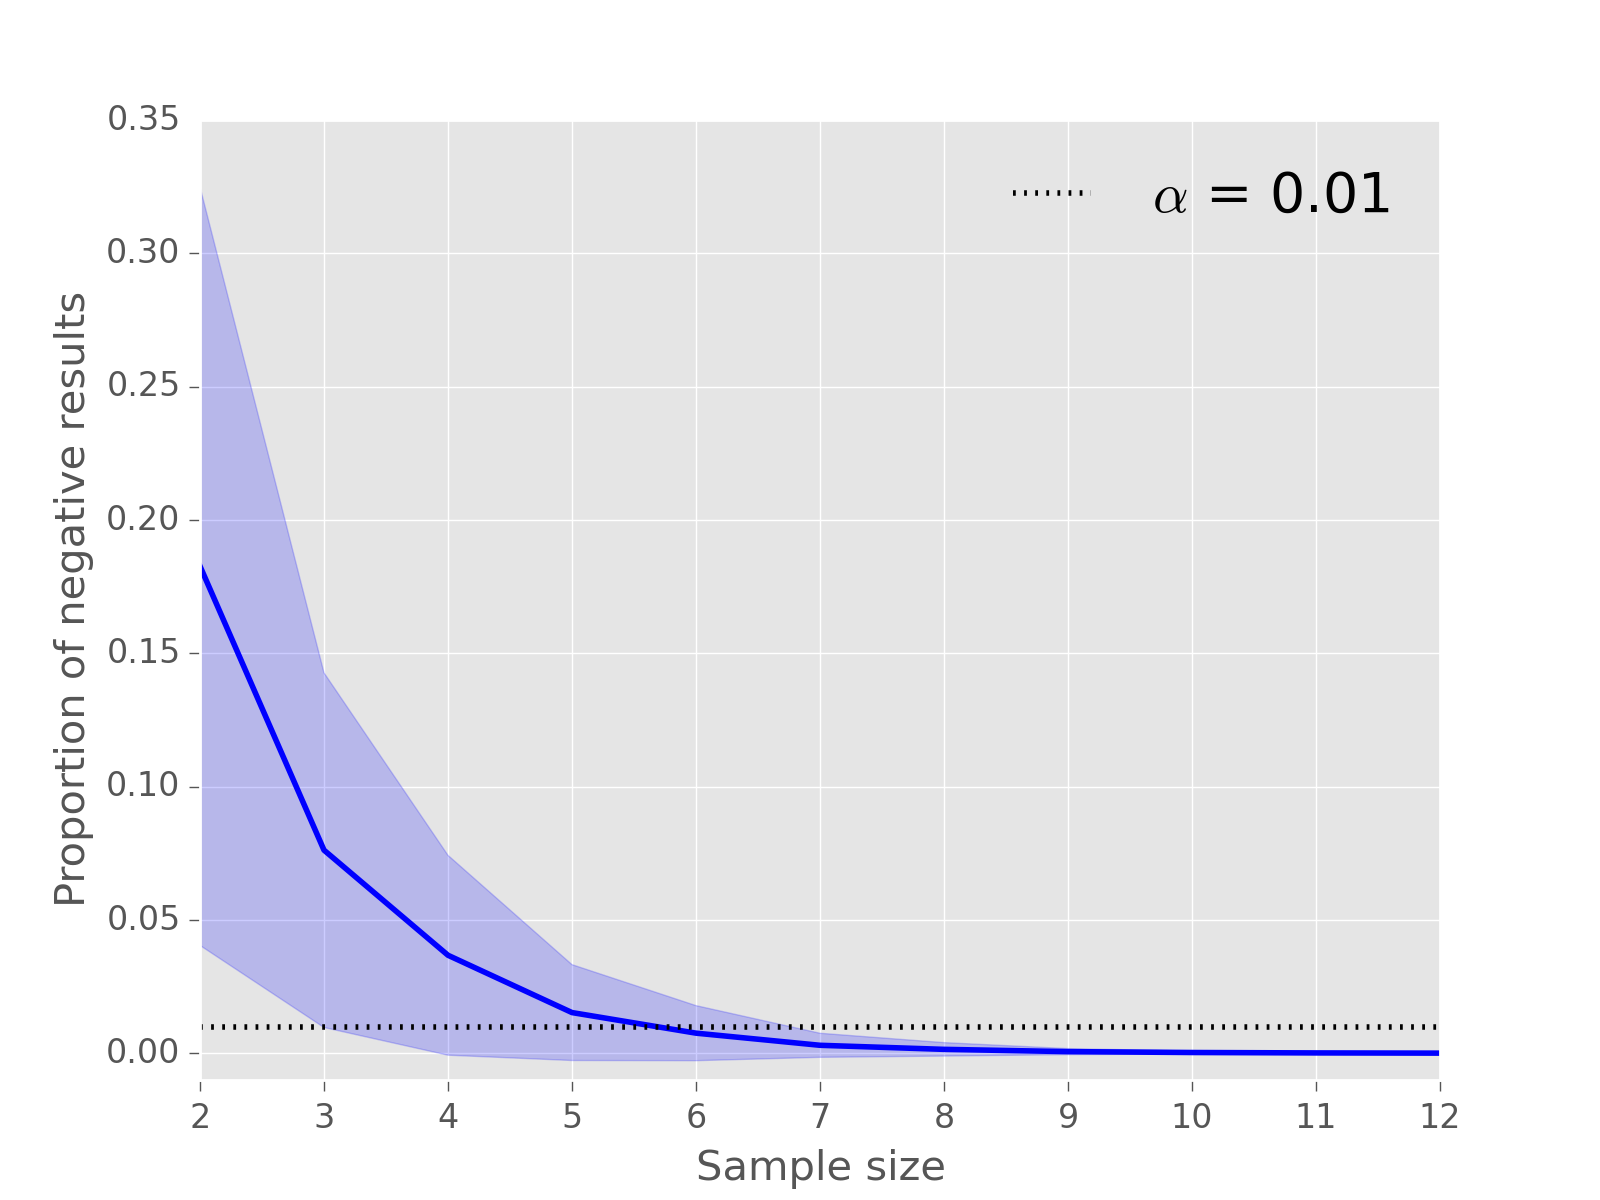
\includegraphics[scale=.7]{bootstrap_results}
\end{figure}

However, it should be noted that the current study's effect size and sampling distribution may not accurately reflect many MVPA studies in the neuroscientific literature, which often contain more subjects and thus a more reliable and robust sample. It is therefore advised to interpret these results with caution and that, ideally, this minimum sample size determination will be validated on different datasets with a larger sample size. 

\newpage
\vspace*{1px}
\subsection{\LARGE \textnormal{Appendix C: Significant within-ROI classification scores}}
\vspace{10px}

\begin{table*}[ht]
%\caption*{\textbf{Table 2}. Overview of ROIs with significant decoding accuracies.}
\begin{threeparttable}
\fontsize{9}{8}\selectfont
\begin{tabular*}{1\textwidth}{l @{\extracolsep{\fill}} lll}
\hline
\textbf{ROI}                     & \textbf{Mean accuracy (SD)} & \textbf{t-value} & \textbf{p-value}\tnote{1} \\ \hline
Temporal Fusiform posterior (L)     & 0.493 (0.058)               & 9.602            & 0.000001         \\
LOC superior (L)                   & 0.569 (0.090)               & 9.113            & 0.000001         \\
Middle frontal gyrus (L)                        & 0.562 (0.087)               & 9.095            & 0.000001         \\
Supramarginal gyrus anterior (L)   & 0.586 (0.097)               & 9.007            & 0.000001         \\
Supramarginal gyrus posterior (L)   & 0.597 (0.104)               & 8.818            & 0.000001         \\
Superior Frontal gyrus (R)                       & 0.526 (0.076)               & 8.791            & 0.000001         \\
Angular gyrus (R)              & 0.541 (0.084)               & 8.593            & 0.000002         \\
Parietal operculum (R)         & 0.514 (0.074)               & 8.440            & 0.000002         \\
Superior parietal lobule (L)     & 0.551 (0.090)               & 8.352            & 0.000002         \\
Temporal pole (R)              & 0.485 (0.064)               & 8.289            & 0.000002         \\
Angular gyrus (L)               & 0.584 (0.106)               & 8.223            & 0.000003         \\
Superior temporal gyrus posterior (L)                  & 0.570 (0.107)               & 7.669            & 0.000005         \\
Temporal fusiform anterior (L)      & 0.433 (0.045)               & 7.659            & 0.000005         \\
Middle frontal gyrus (R)                       & 0.525 (0.087)               & 7.636            & 0.000005         \\
Planum temporale (L)            & 0.558 (0.104)               & 7.485            & 0.000006         \\
Inferior temporal gyrus posterior (L)                  & 0.503 (0.079)               & 7.449            & 0.000006         \\
Parietal operculum (L)          & 0.564 (0.107)               & 7.433            & 0.000007         \\
Middle temporal gyrus anterior (L)                   & 0.478 (0.068)               & 7.396            & 0.000007         \\
LOC inferior (L)                   & 0.553 (0.104)               & 7.365            & 0.000007         \\
Posterior cingulate cortex (L)                        & 0.495 (0.076)               & 7.344            & 0.000007         \\
Frontal pole (R)               & 0.530 (0.093)               & 7.328            & 0.000007         \\
Accumbens (R)                 & 0.417 (0.040)               & 7.255            & 0.000008         \\
Supramarginal gyrus posterior (R) & 0.544 (0.101)               & 7.209            & 0.000009         \\
Superior temporal gyrus anterior (L)                   & 0.500 (0.080)               & 7.195            & 0.000009         \\
Inferior frontal gyrus, pars opercularis (L)       & 0.543 (0.102)               & 7.114            & 0.000010         \\
Postcentral gyrus (L)           & 0.552 (0.107)               & 7.070            & 0.000010         \\
Precuneous (L)            & 0.523 (0.093)               & 7.062            & 0.000010         \\
Paracingulate gyrus (L)         & 0.492 (0.080)               & 6.874            & 0.000013         \\
LOC superior (R)                  & 0.508 (0.089)               & 6.845            & 0.000014         \\
Planum temporale (R)           & 0.513 (0.091)               & 6.840            & 0.000014         \\
Precentral gyrus (L)            & 0.538 (0.105)               & 6.738            & 0.000016         \\
Insular cortex (R)             & 0.435 (0.053)               & 6.666            & 0.000018         \\
Precuneous (R)                & 0.503 (0.088)               & 6.665            & 0.000018         \\
Middle temporal gyrus temporocciptal (L)               & 0.551 (0.113)               & 6.657            & 0.000018         \\
Supplementary motor area (L)                        & 0.506 (0.091)               & 6.582            & 0.000020         \\
Inferior frontal gyrus, pars opercularis (R)      & 0.517 (0.098)               & 6.475            & 0.000023         \\
Superior frontal gyrus (L)                        & 0.539 (0.111)               & 6.428            & 0.000024         \\
Frontal medial cortex (R)       & 0.443 (0.059)               & 6.400            & 0.000025         \\
Superior parietal lobule (R)    & 0.501 (0.092)               & 6.328            & 0.000028         \\
Temporal pole (L)               & 0.486 (0.084)               & 6.318            & 0.000028         \\
Middle temporal gyrus posterior (L)                  & 0.524 (0.105)               & 6.300            & 0.000029         \\
Frontal pole (L)                & 0.537 (0.114)               & 6.203            & 0.000033         \\
Inferior frontal gyrus, pars triangularis (L)      & 0.529 (0.112)               & 6.068            & 0.000041         \\
Precentral gyrus (R)          & 0.513 (0.103)               & 6.063            & 0.000041         \\
Supramarginal gyrus anterior (R)   & 0.514 (0.103)               & 6.055            & 0.000041         \\
Middle temporal gyrus, temporoccipital (R)              & 0.520 (0.107)               & 6.048            & 0.000042         \\
Central operculum (L)           & 0.526 (0.112)               & 5.995            & 0.000045         \\
Inferiof temporal gyrus anterior (L)                   & 0.460 (0.074)               & 5.902            & 0.000051         \\
Middle temporal gyrus posterior (R)                 & 0.491 (0.094)               & 5.838            & 0.000056         \\
Frontal operculum (R)          & 0.468 (0.081)               & 5.760            & 0.000063         \\
Orbitofrontal cortex (R)             & 0.451 (0.071)               & 5.747            & 0.000064         \\
Insular cortex (L)              & 0.473 (0.084)               & 5.730            & 0.000066         \\
Superior temporal gyrus posterior (R)                 & 0.517 (0.112)               & 5.695            & 0.000070         \\
Orbitofrontal cortex (L)              & 0.496 (0.099)               & 5.693            & 0.000070         \\
Intracalcarine cortex (L)       & 0.451 (0.072)               & 5.671            & 0.000072         \\
Supracalcarine cortex (L)       & 0.469 (0.084)               & 5.631            & 0.000077         \\
Parahippocampal cortex anterior (L)       & 0.418 (0.052)               & 5.621            & 0.000078         \\
Anterior cingulate cortex (R)                       & 0.458 (0.077)               & 5.596            & 0.000081         \\
Inferior temporal gyrus, temporoccipital (L)               & 0.494 (0.100)               & 5.585            & 0.000082         \\
Anterior cingulate cortex (L)                        & 0.467 (0.083)               & 5.554            & 0.000086         \\
Superior temporal gyrus anterior (R)                  & 0.460 (0.079)               & 5.532            & 0.000089         \\ \hline

\end{tabular*}
\begin{tablenotes} 
		\item [1] \small{All p-values are significant at $\alpha$ = 0.01, Bonferroni corrected.}
		\end{tablenotes}
\end{threeparttable}
\end{table*}

\newpage
\vspace*{1px}
\subsection{\LARGE \textnormal{Appendix D: Univariate statistical tests of individual ROIs}}
\vspace{10px}

\noindent In the current study we observed that within-ROI average patterns were not sufficient for significant classification accuracy for all but four ROIs, which stands in stark contrast to analyses in which entire within-ROI patterns were used, yielding significant accuracies in over half of the ROIs. To rule out the possibility that multivariate classifiers are less sensitive or otherwise inappropriate to analyse unidimensional data (i.e. scalars representing mean pattern values), we conducted additional univariate analyses on the within-ROI data.

First, we conducted a one-way ANOVA of mean-pattern values in a manner as similar as possible to the multivariate classification analyses. In this analysis, an initial univariate feature selection was performed on the train-data (z-value: 1), which resulting voxel selection was cross-validated on the test-data. Like the multivariate tests, four test-trials per class were used for the independent test-set. For every iteration, mean patterns per test-trial were extracted and submitted to a one-way ANOVA with class as factor. Across 1000 iterations per ROI, we extracted the F-values from the one-way ANOVA. Then, to calculate whether the mean pattern within the ROI differs significantly between classes, we tested the collection of averaged F-values across subjcts to the null-value from the F-distribution, which is 1 (reflecting equal within- and between-condition variance), using a one-sample t-test. Put differently, if the ANOVA within the ROI consistently yields F-values larger than 1, the one-way t-test will likely turn out significant. Similar to the multivariate analyses, we corrected for multiple comparisons using a Bonferroni correction.

Interestingly, none of the ROIs turned out contain significant univariate differences between mean patterns across classes. This observation suggests that multivariate analyses might be more senstitive than univariate analyses \emph{even in case of unidimensional data}. This null-result might, however, be explained by the fact that each iteration used only a small sample size (12 trials) for the univariate analysis (although through iterating this analysis with random subsets of the data, resembling a bootstrapping procedure, should largely mitigate this small sample size and contingent loss of power). Therefore, we conducted another univariate test in which no univariate feature selection was performed, making cross-validation unnecessary and consequently allows to perform, per ROI, a single one-way ANOVA on all trials at once. Again, this yielded no ROIs with significant p-values, indicating that -- again -- multivariate analyses might be more sensitive than univariate in discovering unidimensional differences between classes. More importantly, these control analyses suggest that, indeed, voxel-level representations of high-level information exist within spatially contiguous ROIs in the brain.

\end{document}
